\documentclass[12pt,oneside]{book}
\usepackage{geometry}                		% See geometry.pdf to learn the layout options. There are lots.
\geometry{a4paper}                   			% ... or a4paper or a5paper or ... 
%\geometry{landscape}                		% Activate for for rotated page geometry
%\usepackage[parfill]{parskip}    		% Activate to begin paragraphs with an empty line rather than an indent
\usepackage{graphicx}				% Use pdf, png, jpg, or epsß with pdflatex; use eps in DVI mode
								% TeX will automatically convert eps --> pdf in pdflatex		
\usepackage{amssymb}

\usepackage[spanish]{babel}			% Permite que partes automáticas del documento aparezcan en castellano.
\usepackage[utf8]{inputenc}			% Permite escribir tildes y otros caracteres directamente en el .tex
\usepackage[T1]{fontenc}				% Asegura que el documento resultante use caracteres de una fuente apropiada.

\usepackage{hyperref}				% Permite poner urls y links dentro del documento

\title{Manual de Analizador Lexico}
\author{Manuel Suárez-Veronica Pozo-Alvaro Ortiz}
%\date{}							% Activate to display a given date or no date

\begin{document}
\maketitle
\tableofcontents

\chapter{Introducción}

El libro a continuación es creado como parte de la documentacion del proyecto de Lenguajes de Programacion, un analizador lexico para C. 
En el cual se utilizara el lenguaje de programacion Haskell (lenguaje funcional) para programarlo.

\chapter{El Analizador Lexico}

	%\includegraphics[width=0.8\textwidth]{./imagenes/PantallaPrincipal.png}

	Un analizador léxico o analizador lexicográfico (en inglés scanner) es la primera fase de un compilador consistente en un programa que recibe como entrada el código fuente de otro programa (secuencia de caracteres) y produce una salida compuesta de tokens (componentes léxicos) o símbolos. Estos tokens sirven para una posterior etapa del proceso de traducción, siendo la entrada para el analizador sintáctico (en inglés parser).

	Su principal funciónconsiste en leer los caracteres de entrada y elaborar como salida una secuencia decomponentes léxicos que utiliza el analizador sintáctico para hacer el análisis. Estainteracción, suele aplicarse convirtiendo al analizador léxico en una subrutina ocorrutina del analizador sintáctico. Recibida la orden “Dame el siguientecomponente léxico” del analizador sintáctico, el analizador léxico lee loscaracteres de entrada hasta que pueda identificar el siguiente componente léxico.Estos componentes léxicos representan:

\begin{itemize}

			\item Palabras reservadas
			if, while, do, . . .
			\item identificadores:
			asociados a variables, nombres de funciones, tipos definidos por el usuario, etiquetas,...
			\item operadores:
			= * + - / == > < ! = . . .
			\item símbolos especiales:
			; ( ) [ ] ...
			\item constantes numéricas:
			literales que representan valores enteros, en comaflotante, etc, 982, 0xF678, -83.2E+2,...
			\item constantes de caracteres:
			literales que representan cadenas concretas decaracteres, ...
			\end {itemize}



\chapter{Historia}
En 1958, Strong y otros proponen una solución al problema de que un compilador fuera portable, y esta era dividir al compilador en dos fases “front end” (analiza el programa fuente) y “back end” (genera código objeto para la máquina objeto).

En 1959, Rabin y Scott proponen el empleo de AFD y AFN para el reconocimiento lexicográfico de los lenguajes.

Aparece BNF (Backus-1960, Naur-1963, Knuth-1964) como una guía para el desarrollo del análisis sintáctico.

1959, Sheridan describe un método de parsing de FORTRAN para introducir paréntesis en una expresión.

En los 60’s se desarrollan diversos métodos de parsers ascendentes y descendentes

Floyd más adelante introduce la técnica de precedencia de operadores y uso de funciones de precedencia

1961, se usa por primera vez un parsing descendente recursivo

En los 60’s se estudia el paso de parámetros por nombre, valor y referencia y se incluyen los procedimientos recursivos para Algol 60

Se desarrolla la localización dinámica de datos

1968, se estudia y definen las GLC, los parsers predictivos y la eliminación de recursividad izquierda

1975, aparece LEX generador automático de analizadores léxicos a partir de expresiones regulares bajo UNIX

A mitad de los 70’s Johnson crea YACC para UNIX (generador de analizadores sintácticos)

Ahora un compilador de divide en varias fases

\chapter{Aplicación}
	
	Nuestra aplicación lee un archivo de un código guardado con el nombre cod\_c. El archivo debe tener el codigo separado todas las palabras reservadas, identificadores, operadores y simbolos especiales separados con un espacio. Cuando leemos el archivo, guardamos una lista con todas las palabras (separadas por espacios) y verificamos si se encuentran en el listado de palabras reservadas. Si se encuentra en el listado de palabras reservadas, las guarda en un archivo de texto de esta manera:

	"int, Palabra reservada"

	Luego se verifica si se trata de operadores o simbolos especiales y se guarda de manera similar. Si no es ninguno de los anteriores si asume que es un identificador.

	Ejecutando por linea de comando, nuestra aplicación se ve de esta manera:

	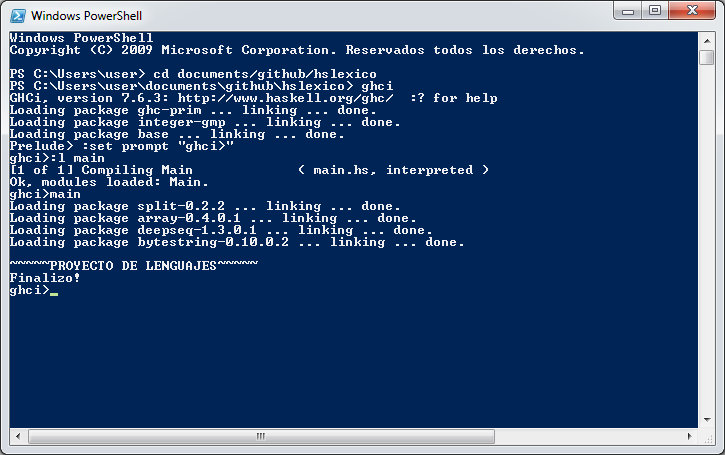
\includegraphics[width=0.4\textwidth]{./imagenes/wps.png}

	
\chapter{Funcionalidad}

\begin{itemize}
\item  Eliminar comentarios

	Antes de separar el archivo en palabras, se eliminan todos los comentarios que esten entre /* */

	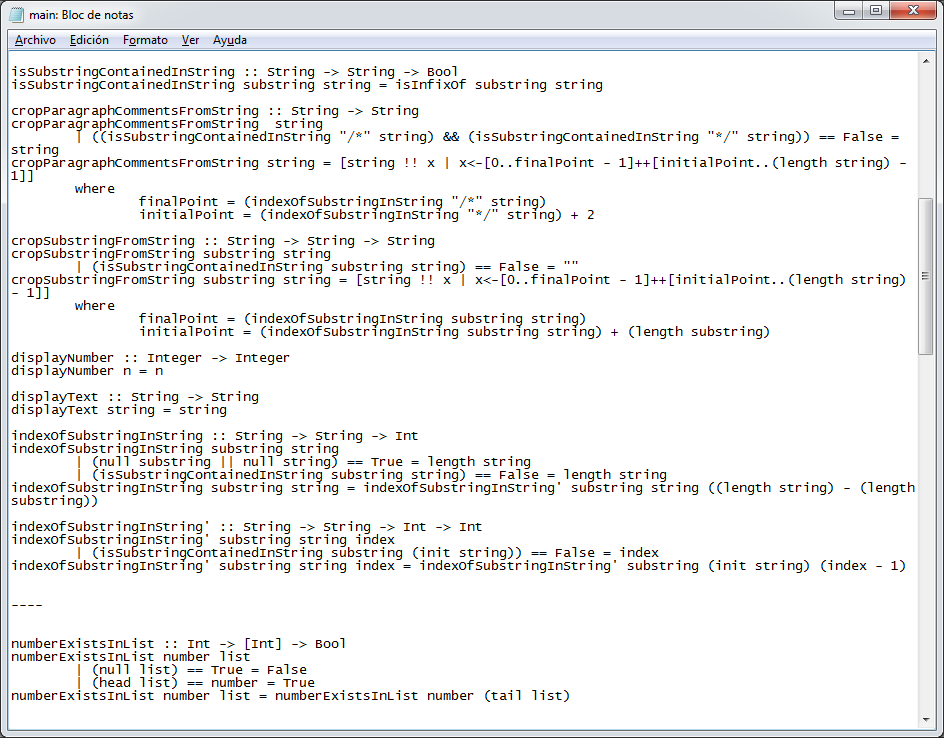
\includegraphics[width=0.55\textwidth]{./imagenes/codigoEliminarComentarios.png}


\item  Análisis Léxico.
	Se separa en una lista todas las palabras. Se verifica palabra por palabra de que tipo se trata. Durante la verificación se guarda el archivo de texto tok.txt con los tokens.

	\includegraphics[width=0.55\textwidth]{./imagenes/codigo.png}

\end{itemize}


\chapter{Colaboraciones}

\begin {itemize}	

\item Commits por integrante.
\begin{itemize}
\item Alvaro Ortiz: 2
\item Veronica Pozo: 2
\item Manuel Suárez: 2

\end{itemize}

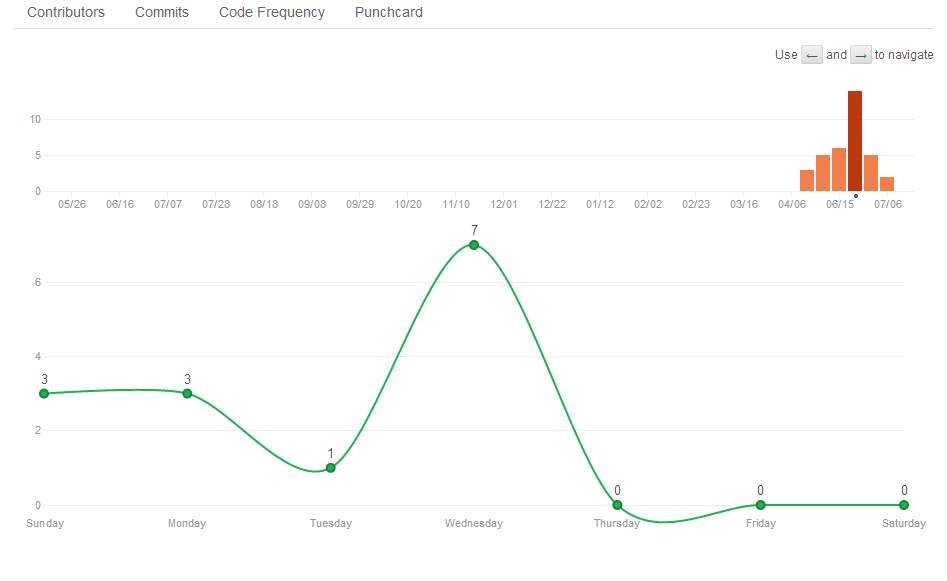
\includegraphics[width=1.10\textwidth]{./imagenes/Contribuidores_linea.png}

\item ¿En qué fechas hay picos?
\begin{itemize}
\item 4 de Septiembre
\end{itemize}
	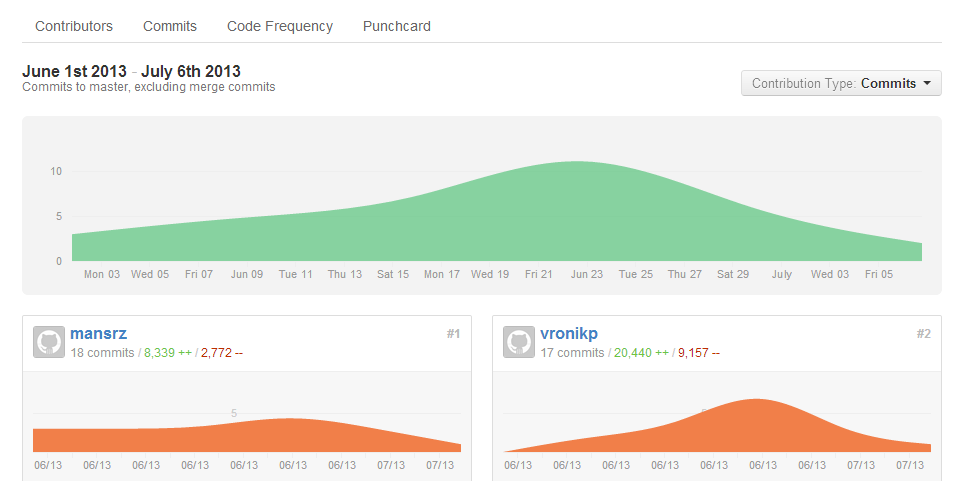
\includegraphics[width=1.10\textwidth]{./imagenes/Contribuidores_commit.png}
\end{itemize}
\chapter{Conclusiones}
El proyecto se realizo con exito logrando implementar la mayoria de caracteristicas en nuestra aplicacion que se pedian. 
Nuestra aplicación permite archivos con comentarios, los cuales son eliminados antes de hacer el analisis. El analisis está limitado por que todas las palabras estén separadas por espacios a excepción de los punteros y numerales.


\end{document}  
